% This report uses the
% LLNCS macro package for Springer Computer Science proceedings;
% Version 2.20 of 2017/10/04
%
\documentclass[runningheads]{llncs}
%
\usepackage{graphicx}
% Used for displaying a sample figure. If possible, figure files should
% be included in EPS format.
%
% If you use the hyperref package, please uncomment the following line
% to display URLs in blue roman font according to Springer's eBook style:
% \renewcommand\UrlFont{\color{blue}\rmfamily}

\begin{document}
%
\title{Coursework 1 - Data Exploration}
%
%\titlerunning{Abbreviated paper title}
% If the paper title is too long for the running head, you can set
% an abbreviated paper title here
%
\author{David Frame}
%
\authorrunning{D. Frame}
% First names are abbreviated in the running head.
% If there are more than two authors, 'et al.' is used.
%
\institute{Edinburgh Napier University\\
\email{40200819@live.napier.ac.uk}}
%
\maketitle              % typeset the header of the contribution
%
\begin{abstract}
In this report, we will discuss 7 relationships found in a data set - and demonstrate them using visualization techniques. We will then dive deeper into the most interesting relationship by optimizing a visualization for clarity and easier understanding.

%The abstract should briefly summarize the %contents of the paper in
%150--250 words.

%\keywords{First keyword  \and Second keyword %\and Another keyword.}
\end{abstract}
%
%
% DESCRIPTION OF RELATIONSHIPS
\section{Description of the relationships found}

To find the 7 relationships, graphs were created by plotting various attributes against each other. 

For efficiency, facet wraps were used to check each combination of qualitative variables against each combination of quantitative variables.

By doing this, some relationships were found in the data which are detailed in the following subsections.

\subsection{Jump scores improve with age for women}

%Please note that the first paragraph of a %section or subsection is
%not indented. The first paragraph that follows %a table, figure,
%equation etc. does not need an indent, either.

%Subsequent paragraphs, however, are indented.

When looking at overall scores against age on a box plot, it becomes clear that over 30s have a better overall score than the other age groups.

Two relationships can be found in the data that explain the higher overall score of this age group - the first relating to jump scores for females.

As figure~\ref{jumAgeWomen} shows, each age group's box plot is above the previous, indicating that female jump scores get higher with age. Therefore, the over 30s age group has the highest score as it is the oldest group in the data set.

\subsection{Over 30s have the highest distance scores}

The second relationship contributing to the higher overall score for over 30s involves distance scores, which are higher for over 30s than any other age group.

In figure \ref{ageDist}, the over 30s box plot is above all the others, showing the clear strength of the age group in this category.

\subsection{Location D has a higher overall score than the other locations}
When looking at a box-plot of location vs overall score (see figure \ref{overLoc}), location D has a higher box than all of the other locations.

%\subsection{The relationship between sprint and distance scores is interesting}
%These two variables have a fluctuating relationship initially, before starting toward a steady positive correlation as the scores approach 100.

%This is a relationship - There is a similar correlation between sprint and jump scores, although they settle to a steady positive correlation much quicker and it is a much stronger correlation.

%Finally is the relationship between distance and jump, which is a negative correlation at first, before sharply changing to a very strong positive correlation after the halfway point and another sharp drop-off near a score of 100.

\subsection{There is a strong correlation between throw and sprint scores for locations A and C}
There is a strong negative correlation between the throw and sprint scores of people from locations A and C.

Looking at the scatter plot for location A (see figure \ref{throwSprintLocA}), there is a clear line showing a 1:1 negative correlation.

\subsection{Distance and jump scores have a quadratic relationship for men in location B}

When plotting distance score against jump score for men in location B, there is a clear quadratic curve (see figure \ref{distJumpLocBMen}) - showing a negative correlation until a score of 50 for distance, then flipping to a positive correlation.

\subsection{Female teens from location E have a strong positive correlation between sprint and jump scores}
As figure \ref{fTeSprintJump} shows, There is a 1:1 positive correlation between jump and sprint scores for female teens from location E.

\subsection{Overall scores improve with jump scores for men, especially in locations A and C}
Figure \ref{menACjumover} shows that male overall scores improve as their jump scores do - with an especially strong correlation if they are from locations A or C. This could be related to the relationship between throw and sprint scores (see figure \ref{throwSprintLocA}) as it involves the same two locations.

%\subsubsection{Sample Heading (Third Level)} %Only two levels of
%headings should be numbered. Lower level %headings remain unnumbered;
%they are formatted as run-in headings.

%\paragraph{Sample Heading (Fourth Level)}
%The contribution should contain no more than %four levels of
%headings. Table~\ref{tab1} gives a summary of %all heading levels.

%\begin{table}
%\caption{Table captions should be placed above the
%tables.}\label{tab1}
%\begin{tabular}{|l|l|l|}
%\hline
%Heading level &  Example & Font size and style\\
%\hline
%Title (centered) &  {\Large\bfseries Lecture Notes} & 14 point, bold\\
%1st-level heading &  {\large\bfseries 1 Introduction} & 12 point, bold\\
%2nd-level heading & {\bfseries 2.1 Printing Area} & 10 point, bold\\
%3rd-level heading & {\bfseries Run-in Heading in Bold.} Text follows & 10 point, bold\\
%4th-level heading & {\itshape Lowest Level Heading.} Text follows & 10 point, italic\\
%\hline
%\end{tabular}
%\end{table}


%\noindent Displayed equations are centered and set on a separate
%line.
%\begin{equation}
%x + y = z
%\end{equation}
%Please try to avoid rasterized images for line-art diagrams and
%schemas. Whenever possible, use vector graphics instead (see
%Fig.~\ref{fig1}).

\section{Most interesting relationship}
When finding the relationships listed above, the quadratic relationship between distance and jump scores for men in location B (shown in figure \ref{distJumpLocBMen}) stood out. Figure \ref{distJumpLocBMenOpt} shows an optimized visualization that should make the relationship more obvious and clear.

To effectively optimize this relationship, the data was filtered to only include men and location B. This helped remove a lot of noise and gave an almost perfect quadratic curve. Adding a line of best fit further emphasized the curve. The axis were renamed from 'sj' and 'sd' to 'Jump Score' and 'Distance Score' and the graph was given an appropriate title.

After referring to some of the literature \cite{effcomnum}, the grid lines were excluded as they would have obscured the curve that needed to be the focus of the visualization. Black axis lines were added to better frame the graph and to keep the axis separate from the graph itself. The background was made white to improve the contrast, making the curve blatantly obvious. To accomplish this, a tutorial website hosted on GitHub was used \cite{remGridBack}.

The graph doesn't show values below 30 or above 80 on the y (Jump Score) axis. This was due to a default setting from ggplot2 that hides space when no data is present, but it wasn't changed as it emphasized the curve even further.

Removing the points and just using a line was considered, but it became clear that the points are perfectly symmetrical around the center of the X axis, which shows that the curve isn't just a line of best fit that looks symmetrical, it actually is symmetrical. A paper about graphical excellence also influenced the decision not to simplify the graph too much, instead encouraging the use of points to represent data more honestly than a line of best fit can \cite{graphExcellence}.

After finding the symmetrical data, a table was considered for inclusion in the visualization - ordered to make the symmetrical nature of the data clear and numerical - but it was decided against when considering the size of the data set, which was 1000 rows.

\bibliographystyle{splncs04}
\bibliography{mybibliography}
%

\begin{thebibliography}{8}
\bibitem{effcomnum}
Few, Stephen.: Effectively Communicating Numbers: Selecting the Best Means and Manner of Display. p. 22 (2005)

\bibitem{remGridBack}
Dealing with grid lines and backgrounds, \url{http://felixfan.github.io/ggplot2-remove-grid-background-margin/}.

\bibitem{graphExcellence}
Tufte, Edward R..: The Visual Display of Quantitative Information. 2nd edn. Graphics Press USA,
(2001)

\end{thebibliography}
\newpage
\section{Visualizations}

\begin{figure}[h!]
\begin{multicols}{2}
    % Jump Age Women %
    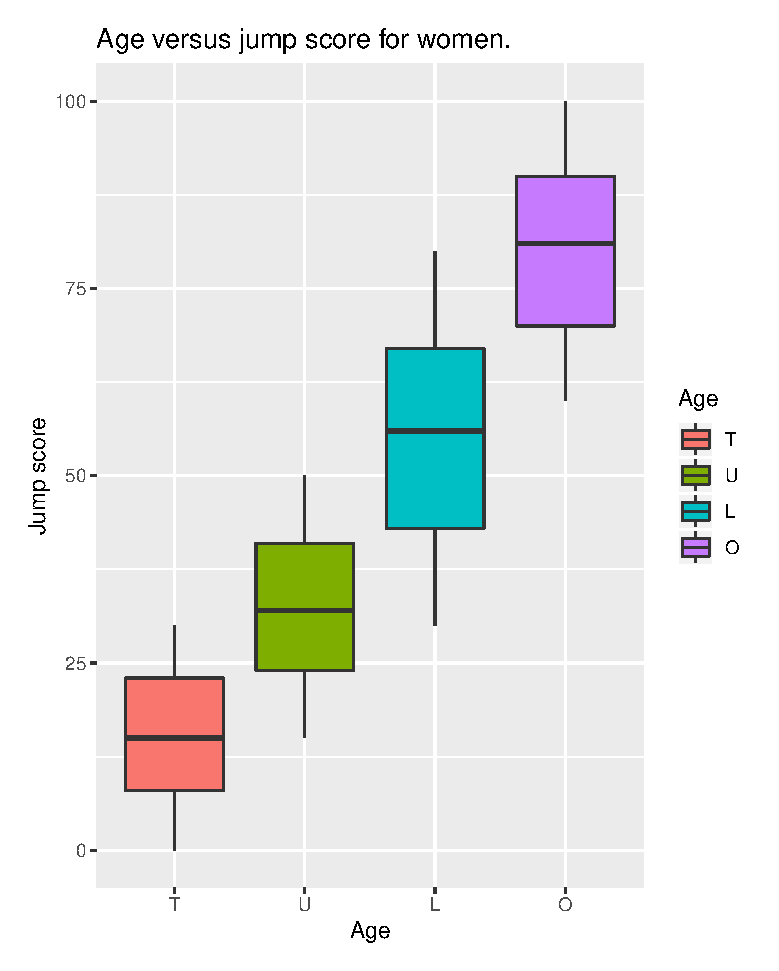
\includegraphics[width=\linewidth]{jumAgeWomen.eps} \vspace{-0.7cm} \caption{Each box-plot represents a different age group.} \label{jumAgeWomen} \par
    
    % Age distance %
    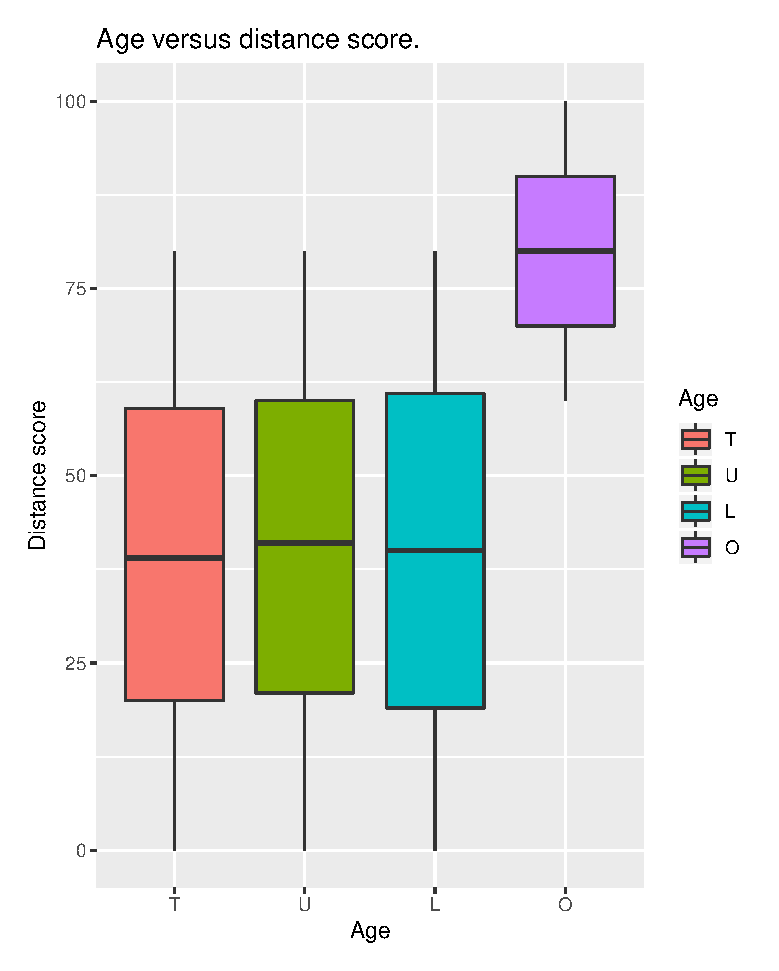
\includegraphics[width=\linewidth]{AgeDist.eps} \vspace{-0.7cm} \caption{The over 30s box plot, shown in purple, is above all of the others.} \label{ageDist} \par
\end{multicols}   
\begin{multicols}{2}
    % Overall location
    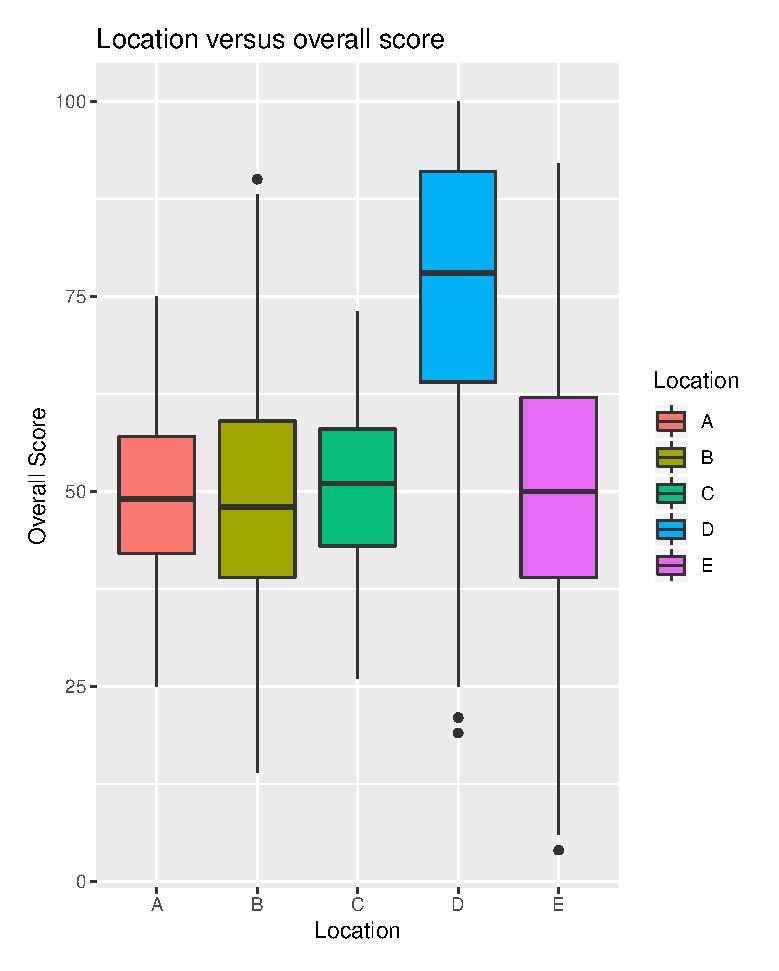
\includegraphics[width=\linewidth]{overLoc.eps} \vspace{-0.7cm} \caption{The blue box plot, representing location D, is higher than the others.} \label{overLoc} \par
    
    % Distance Jump Location A
    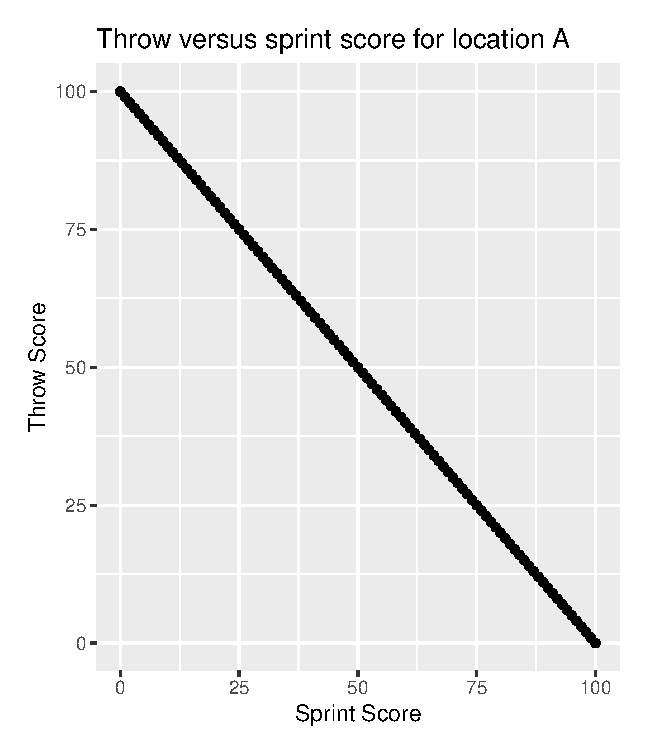
\includegraphics[width=\linewidth]{throwSprintLocA.eps} \vspace{-0.7cm} \caption{There is a 1:1 negative correlation between throw and sprint scores.} \label{throwSprintLocA} \par
\end{multicols} 
\end{figure}
\begin{figure}
\begin{multicols}{2}
    % Distance Jump Location B Men
    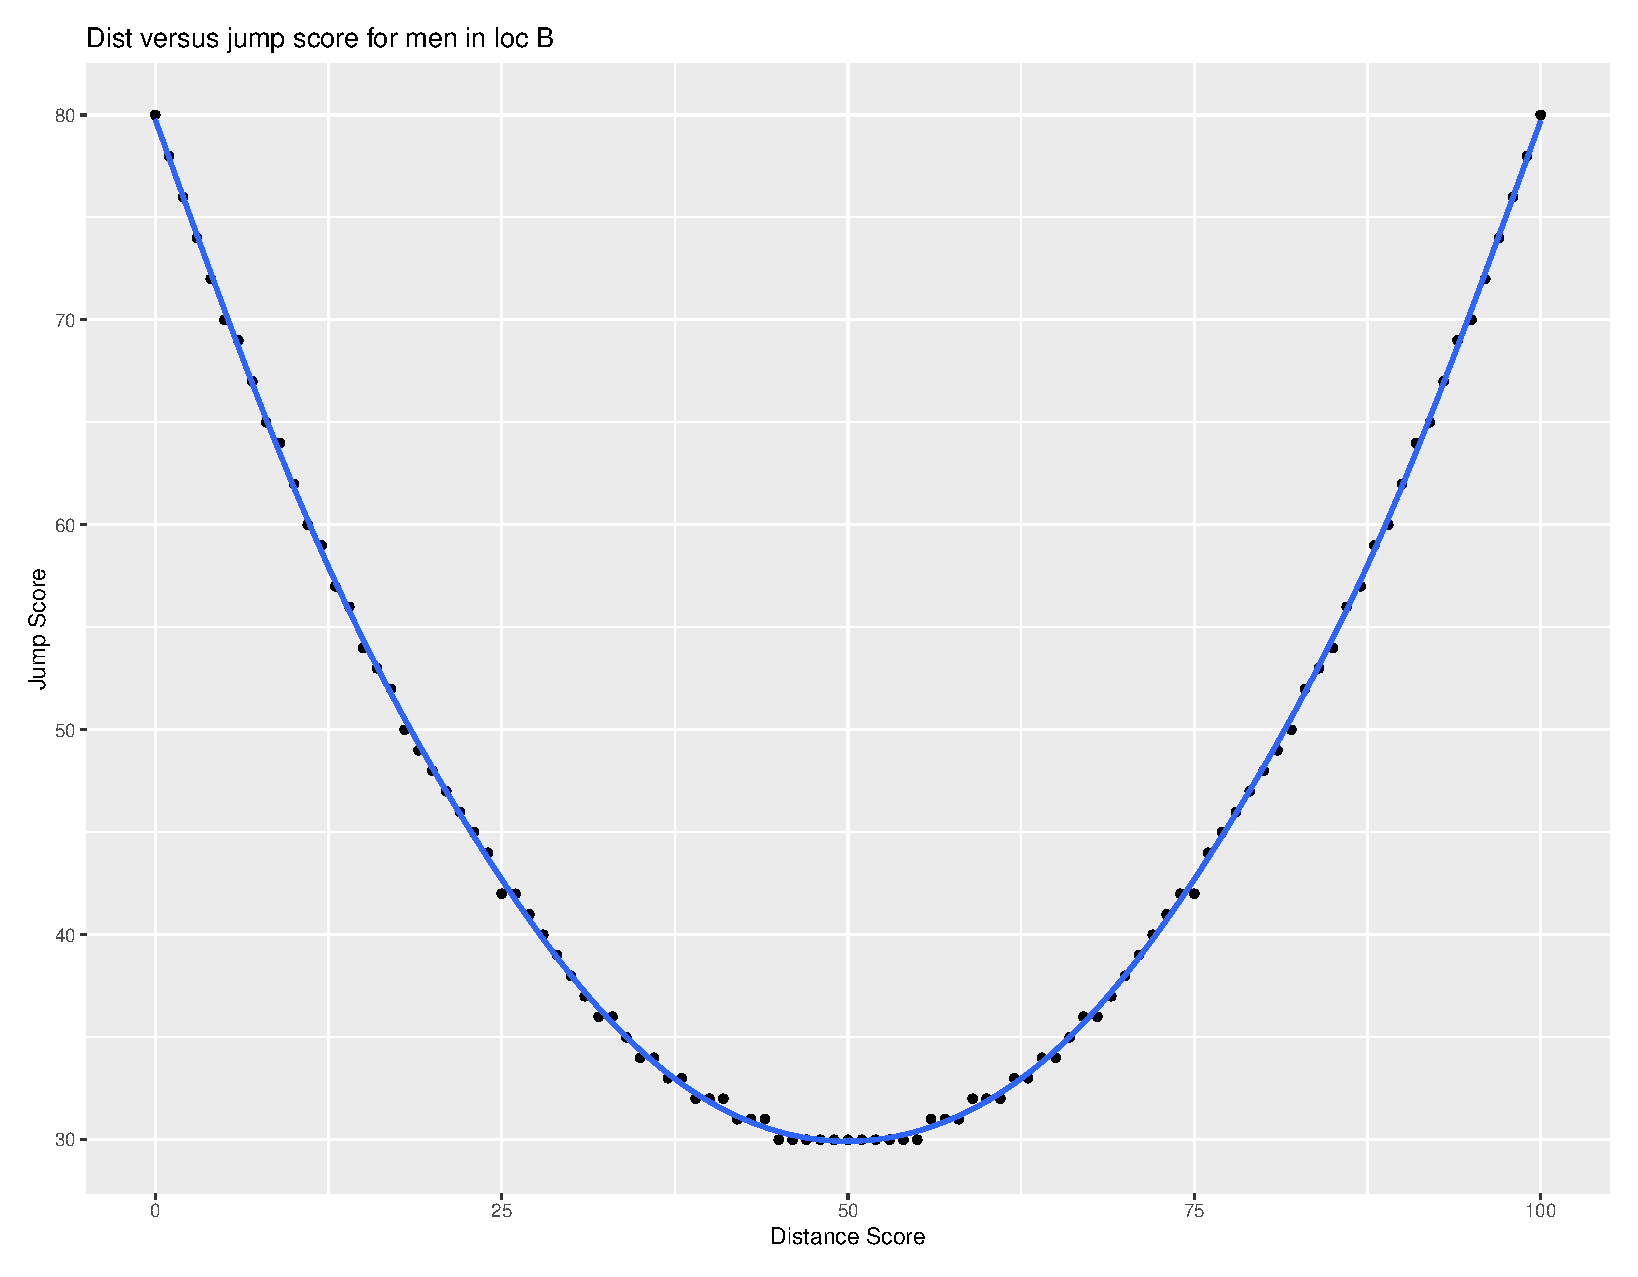
\includegraphics[width=\linewidth]{distJumpLocBMen.eps} \vspace{0cm} \caption{There is a quadratic relation between distance and jump scores.} \label{distJumpLocBMen} \par
    
    %Sprint jump Female Teen Location E
    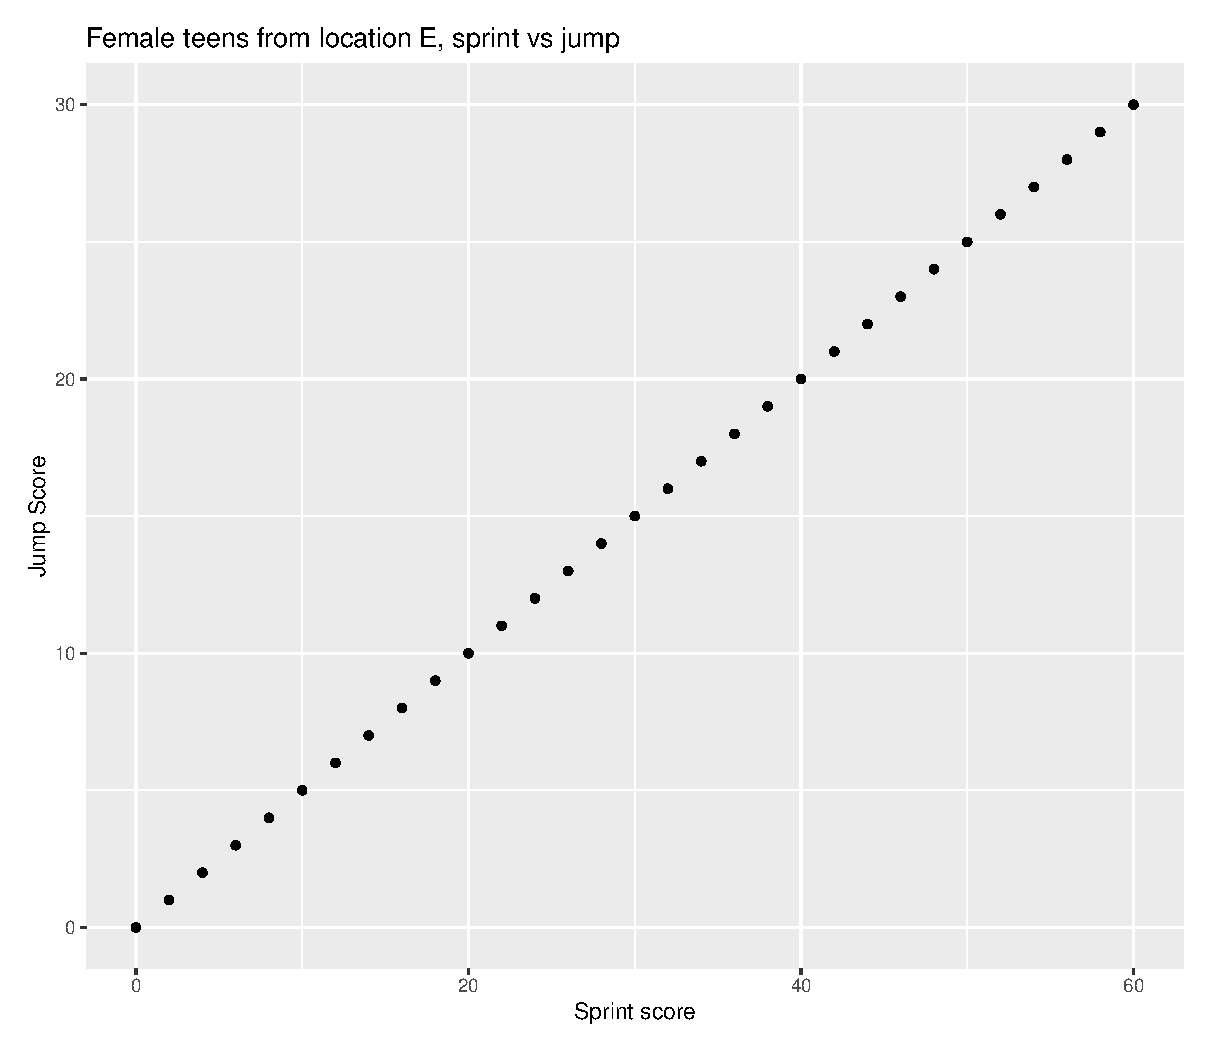
\includegraphics[width=\linewidth]{fTeSprintJump.eps} \vspace{-0.7cm} \caption{There is a strong positive correlation between sprint and jump for female teens in location E.} \label{fTeSprintJump} \par
\end{multicols}
\begin{multicols}{2}
    %Male Sprint Overall Facet Wrap
    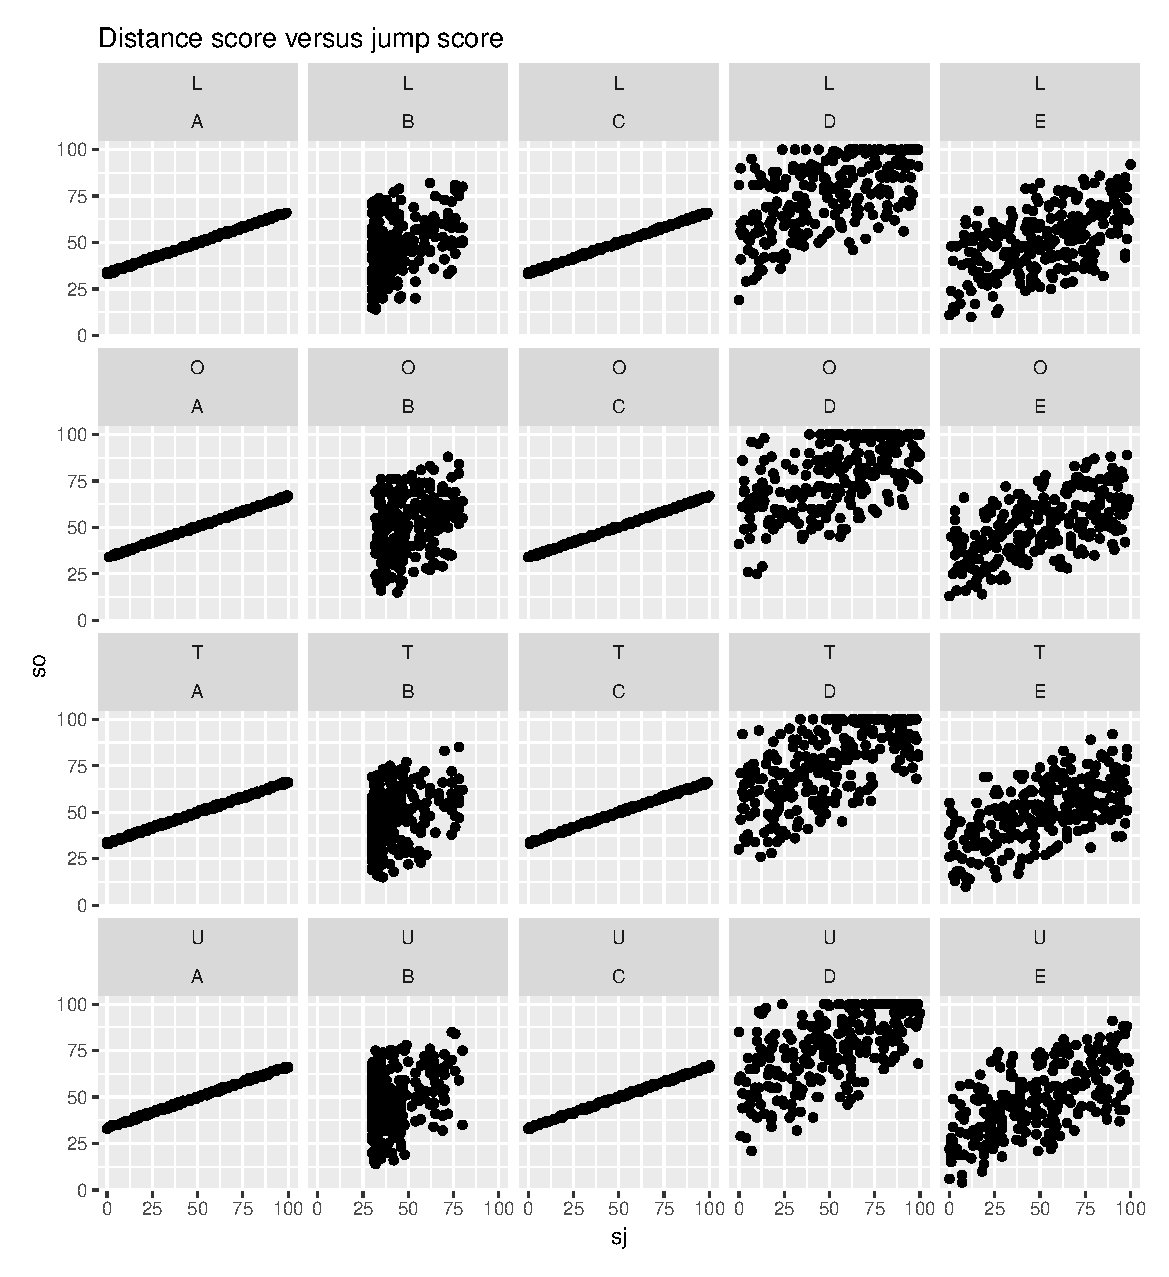
\includegraphics[width=\linewidth]{menACjumover.eps} \vspace{-0.8cm} \caption{There is a positive correlation between jump and overall scores for men, especially those from locations A and C.} \label{menACjumover} \par

    %Distance Jump Location B Men OPTIMIZED
    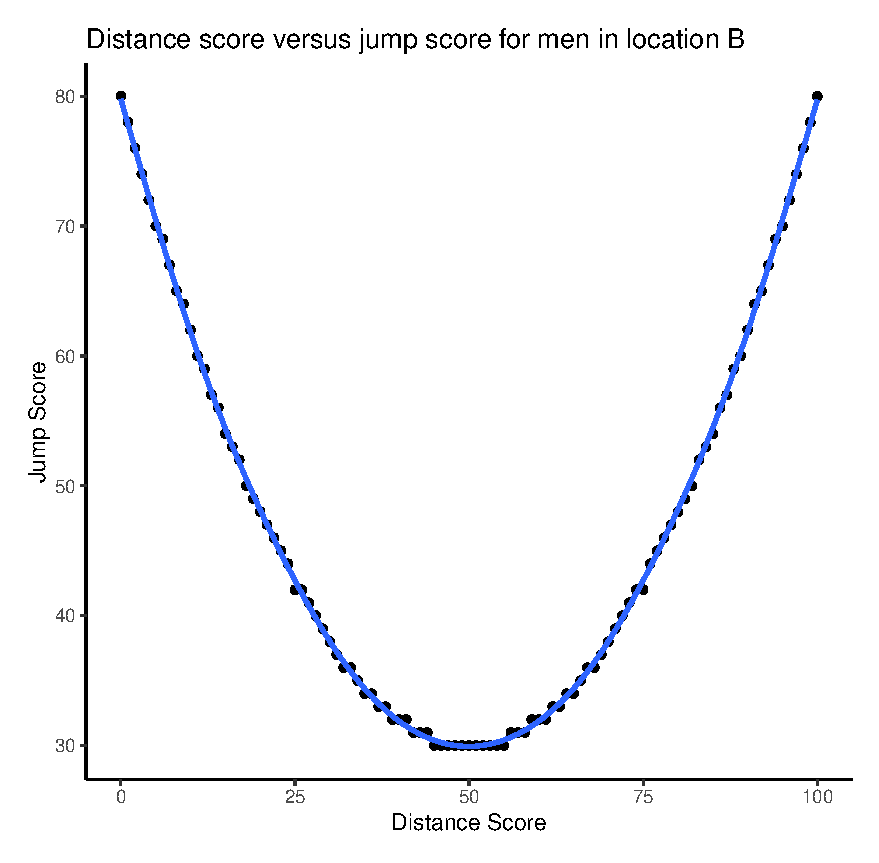
\includegraphics[width=\linewidth]{distJumpLocBMenOpt.eps} \vspace{-0.8cm} \caption{The optimized version of figure \ref{distJumpLocBMen}. As the original was already quite clear, I mostly focused on removing background elements for this optimized version.} \label{distJumpLocBMenOpt} \par

\end{multicols}
\end{figure}
%
% the environments 'definition', 'lemma', 'proposition', 'corollary',
% 'remark', and 'example' are defined in the LLNCS documentclass as well.
%
%\begin{proof}
%Proofs, examples, and remarks have the initial word in italics,
%while the following text appears in normal font.
%\end{proof}
%For citations of references, we prefer the use of square brackets
%and consecutive numbers. Citations using labels or the author/year
%convention are also acceptable. The following bibliography provides
%a sample reference list with entries for journal
%articles~\cite{ref_article1}, an LNCS chapter~\cite{ref_lncs1}, a
%book~\cite{ref_book1}, proceedings without editors~\cite{ref_proc1},
%and a homepage~\cite{ref_url1}. Multiple citations are grouped
%\cite{ref_article1,ref_lncs1,ref_book1},
%\cite{ref_article1,ref_book1,ref_proc1,ref_url1}.

\end{document}
